% Instructions to modify this document:
% * Remember to ALWAYS execute "git pull" BEFORE any commit you make!
% * Use the \ToDo{...} command to remark tasks which still need to be done. Add your name in the comment.
% * Use the \input{file.tex} command to split the document into several parts
% * Do not change the current LaTeX coding style to yours. The style and format should be homogeneous along sections.

% To convert .dia diagrams into PDF:
% 1) Create the diagram with dia
% 2) Export it as .eps
% 3) use epstopdf to convert to PDF
%
% Editing SVG files and exporting them to PDF with Inkscape is admitted too.
% Remember to keep a copy of the editable file (.dia or .svg files).


\documentclass[a4paper,12pt]{article}

\usepackage[utf8]{inputenc}
\usepackage{amsmath,graphicx}
\usepackage{bm}
\usepackage{amssymb}
\usepackage{algorithm}
\usepackage{algpseudocode}
\usepackage{subfigure}
\usepackage{ifpdf}
\usepackage[hyphens]{url}
\usepackage{color}
\usepackage[hidelinks]{hyperref}
\usepackage{multirow}
\usepackage{datetime}
\usepackage{comment}
\usepackage{float} % To put figures in their exact place with \begin{figure}[H]
\usepackage{longtable}
\usepackage{tabularx}
\usepackage{listings}
\usepackage{xcolor}
\usepackage{color}

\definecolor{mygreen}{rgb}{0,0.6,0}
\definecolor{mygray}{rgb}{0.5,0.5,0.5}
\definecolor{mymauve}{rgb}{0.58,0,0.82}

\lstset{ %
  language=HTML,                 % the language of the code
  backgroundcolor=\color{white},   % choose the background color; you must add \usepackage{color} or \usepackage{xcolor}
  basicstyle=\small,        % the size of the fonts that are used for the code
  breakatwhitespace=false,         % sets if automatic breaks should only happen at whitespace
  breaklines=true,                 % sets automatic line breaking
  captionpos=b,                    % sets the caption-position to bottom
  commentstyle=\color{mygreen},    % comment style
  deletekeywords={...},            % if you want to delete keywords from the given language
  escapeinside={\%*}{*)},          % if you want to add LaTeX within your code
  extendedchars=true,              % lets you use non-ASCII characters; for 8-bits encodings only, does not work with UTF-8
  frame=single,                    % adds a frame around the code
  keepspaces=true,                 % keeps spaces in text, useful for keeping indentation of code (possibly needs columns=flexible)
  keywordstyle=\color{blue},       % keyword style
  language=HTML,                 % the language of the code
  otherkeywords={*,...},           % if you want to add more keywords to the set
  numbers=left,                    % where to put the line-numbers; possible values are (none, left, right)
  numbersep=5pt,                   % how far the line-numbers are from the code
  numberstyle=\tiny\color{mygray}, % the style that is used for the line-numbers
  rulecolor=\color{black},         % if not set, the frame-color may be changed on line-breaks within not-black text (e.g. comments (green here))
  showspaces=false,                % show spaces everywhere adding particular underscores; it overrides 'showstringspaces'
  showstringspaces=false,          % underline spaces within strings only
  showtabs=false,                  % show tabs within strings adding particular underscores
  stepnumber=2,                    % the step between two line-numbers. If it's 1, each line will be numbered
  stringstyle=\color{mymauve},     % string literal style
  tabsize=2,                     % sets default tabsize to 2 spaces
  title=\lstname                   % show the filename of files included with \lstinputlisting; also try caption instead of title
}


\definecolor{lightgray}{rgb}{.9,.9,.9}
\definecolor{darkgray}{rgb}{.4,.4,.4}
\definecolor{purple}{rgb}{0.65, 0.12, 0.82}
\lstdefinelanguage{JavaScript}{
  keywords={break, case, catch, continue, debugger, default, delete, do, else, false, finally, for, function, if, in, instanceof, new, null, return, switch, this, throw, true, try, typeof, var, void, while, with},
  morecomment=[l]{//},
  morecomment=[s]{/*}{*/},
  morestring=[b]',
  morestring=[b]",
  ndkeywords={class, export, boolean, throw, implements, import, this},
  keywordstyle=\color{blue}\bfseries,
  ndkeywordstyle=\color{darkgray}\bfseries,
  identifierstyle=\color{black},
  commentstyle=\color{purple}\ttfamily,
  stringstyle=\color{red}\ttfamily,
  sensitive=true
}

\newcolumntype{L}[1]{>{\raggedright\arraybackslash}p{#1}}
\newcolumntype{C}[1]{>{\centering\arraybackslash}p{#1}}
\newcolumntype{R}[1]{>{\raggedleft\arraybackslash}p{#1}}


% Definitions and commands
\def \np{\vskip 0.25 cm}
\def \ap{\vskip 0.15 cm}

% JSON listing (see 
%  http://tex.stackexchange.com/questions/83085/how-to-improve-listings-display 
% -of- json-files)
\colorlet{punct}{red!60!black}
\definecolor{background}{HTML}{EEEEEE}
\definecolor{delim}{RGB}{20,105,176}
\colorlet{numb}{magenta!60!black}

\lstdefinelanguage{json}{
    basicstyle=\footnotesize\ttfamily,
    numbers=left,
    numberstyle=\scriptsize,
    stepnumber=1,
    numbersep=8pt,
    showstringspaces=false,
    breaklines=true,
    frame=lines,
    backgroundcolor=\color{background},
    literate=
     *{0}{{{\color{numb}0}}}{1}
      {1}{{{\color{numb}1}}}{1}
      {2}{{{\color{numb}2}}}{1}
      {3}{{{\color{numb}3}}}{1}
      {4}{{{\color{numb}4}}}{1}
      {5}{{{\color{numb}5}}}{1}
      {6}{{{\color{numb}6}}}{1}
      {7}{{{\color{numb}7}}}{1}
      {8}{{{\color{numb}8}}}{1}
      {9}{{{\color{numb}9}}}{1}
      {:}{{{\color{punct}{:}}}}{1}
      {,}{{{\color{punct}{,}}}}{1}
      {\{}{{{\color{delim}{\{}}}}{1}
      {\}}{{{\color{delim}{\}}}}}{1}
      {[}{{{\color{delim}{[}}}}{1}
      {]}{{{\color{delim}{]}}}}{1},
}


\newcommand{\ToDo}[1]{\textcolor{magenta}{\textbf{[ToDo]} \textbf{#1}}}
\newcommand{\miguel}[1]{\textcolor{magenta}{\textbf{[Miguel]} \textbf{#1}}}


\begin{document}


\begin{titlepage}

\begin{center}
\vspace*{-1in}

\vspace*{0.6in}
\begin{Large}
\textbf{The IPOL Demo Web interface} \\
\end{Large}

\vspace*{0.6in}

\small{Compiled on \today\ at \currenttime}

\vspace*{0.6in}
\rule{80mm}{0.1mm}\\
\vspace*{0.1in}
\end{center}

\end{titlepage}

This document contains the technical documentation for the Demo Web interface 3.0 that lets the user test demos and their results. This interface provides utility controlls such as inpainting blob editing, image cropping, zoom and blob reproduction.

\vspace*{0.6in}

%\maketitle
\newpage

\tableofcontents
\newpage
\listoffigures
\newpage

% The Demo Description Lines (DDL) and automatic demo generation
\section{IPOL web interface}

current version is 3.0.

\subsection{Introduction}
The IPOL Demo Web Interface has been developed with HTML5, CSS3, and JQuery. 
It allows the users to execute the IPOL algorithms with an ergonomic interface. The users can use their own data or the examples offered by each of the demos. We shall describe the modules of which the web interface is made, its flow diagram, how the asynchronous calls work, and the data types accepted.

\section{Modules}
The Javascript application is made of the following modules:

\begin{itemize}
	\item Inputs
	\item Upload
	\item Editor
	\item Parameters
	\item Run
	\item Results
	\item Helpers 
\end{itemize}

Each of them is described in the following sections.

\subsection{Inputs}
This module manages the list of blobs used as examples in the demo and renders them on the web page. This module is the first which is loaded and it communicates with the DemoInfo and Blobs modules, see Fig. \ref{fig:server_interaction}. Note that neither the web interface nor any of the modules in the IPOL's architecture of microservices need to know of the existence of any module. Instead, a generic API providing services are used, without the need to reach a particular endpoint. The details of the back-end architecture are hidden to both the interface and other modules.

This Inputs module allows the user to choose one or many blobs in the demo. These blobs can be for example images, videos, or audio files. It displays a line of blobs or sets of blobs to choose from.


\subsection{Upload}
If the users want to use their own blobs for the demo this module lets you upload them. Every demo has predefined 
upload slots each with their own characteristics like maximum file size and maximum image size. The user is able to upload the 
minimum required number of uploads. This module listens for events in every upload slot and gets the file information in order to 
upload them when the run button is pressed.


\subsection{Editor}
This module loads after the user selects a set of blobs to run the demo with or when the users upload their blobs. It loads a view of
the chosen blobs where there is a zoom and crop functions when the sets have one blob per set. When the sets have more than 
one blob per set, the user will have the possibility to compare them with the corresponding 'Compare button', but not a crop 
an area.

\subsubsection{Interactive controls}
When an interactive control is specified in the DDL, the appropriate controls will appear under the blob list, adding the hability to draw on top of the blob. The behaviour will depend on the type of control specified. 

Mask control will enable free drawing on top of the selected blob, color change and an eraser tool and will result in an image containing only the drawn strokes and transparent background.

Dots control will display drawings in the form of dots on the canvas. An option is available to limit the number of allowed drawn dots on the canvas wich when reached will substitute the first drawn point when drawing a new one.

The lines control has the only difference when compared to the dots control,  the way the drawing is displayed on the screen connecting the dots drawn in the canvas, everything else is will remain the same. Additionally this control will allow for the drawn lines to close the drawn figure.

\subsection{Parameters}
This module renders the parameters of the demo described in the DDL after the user chooses blobs to use with the demo. 
Parameters have as many types DDL specifies, so the interface renders each type accordingly.

\subsection{Run}
This module will send all the blobs and requirements needed to run the demo on the servers and will send this information to 
the core module. The answer will be either a success message with enough information to render the results or an error message 
that will show an approximation of what failed during execution.

\subsection{Results}
This module renders the results returned by the core letting the user compare the input and results, based on the DDL results section. 
It will use the DDL results section and the data returned by the run call with the execution results. These results include:

\begin{itemize}
	\item gallery: a gallery with compare capabilities
	\item gallery\textunderscore new: A gallery with evaluation, repeat, visibility capabilities
	\item repeat\textunderscore gallery: A gallery with repeat capabilities
	\item file\textunderscore download: file download result
	\item html\textunderscore text: HTML snippet to add in the results view
	\item text\textunderscore file: text file dump in the results view
	\item message: message with custom styling
\end{itemize}

All of these result types are defined in the DDL documentation.


\subsection{Helpers}
This module acts as an interface for common utility methods like reading and writing to sessionStorage, make HTTP requests and 
read the origin of the chosen blobs for the demo, this could be blobset, meaning blobs are chosen from the ones offered by the 
demo, and upload, meaning the user has uploaded his own blobs.

\begin{figure}[ht]
	\centering
	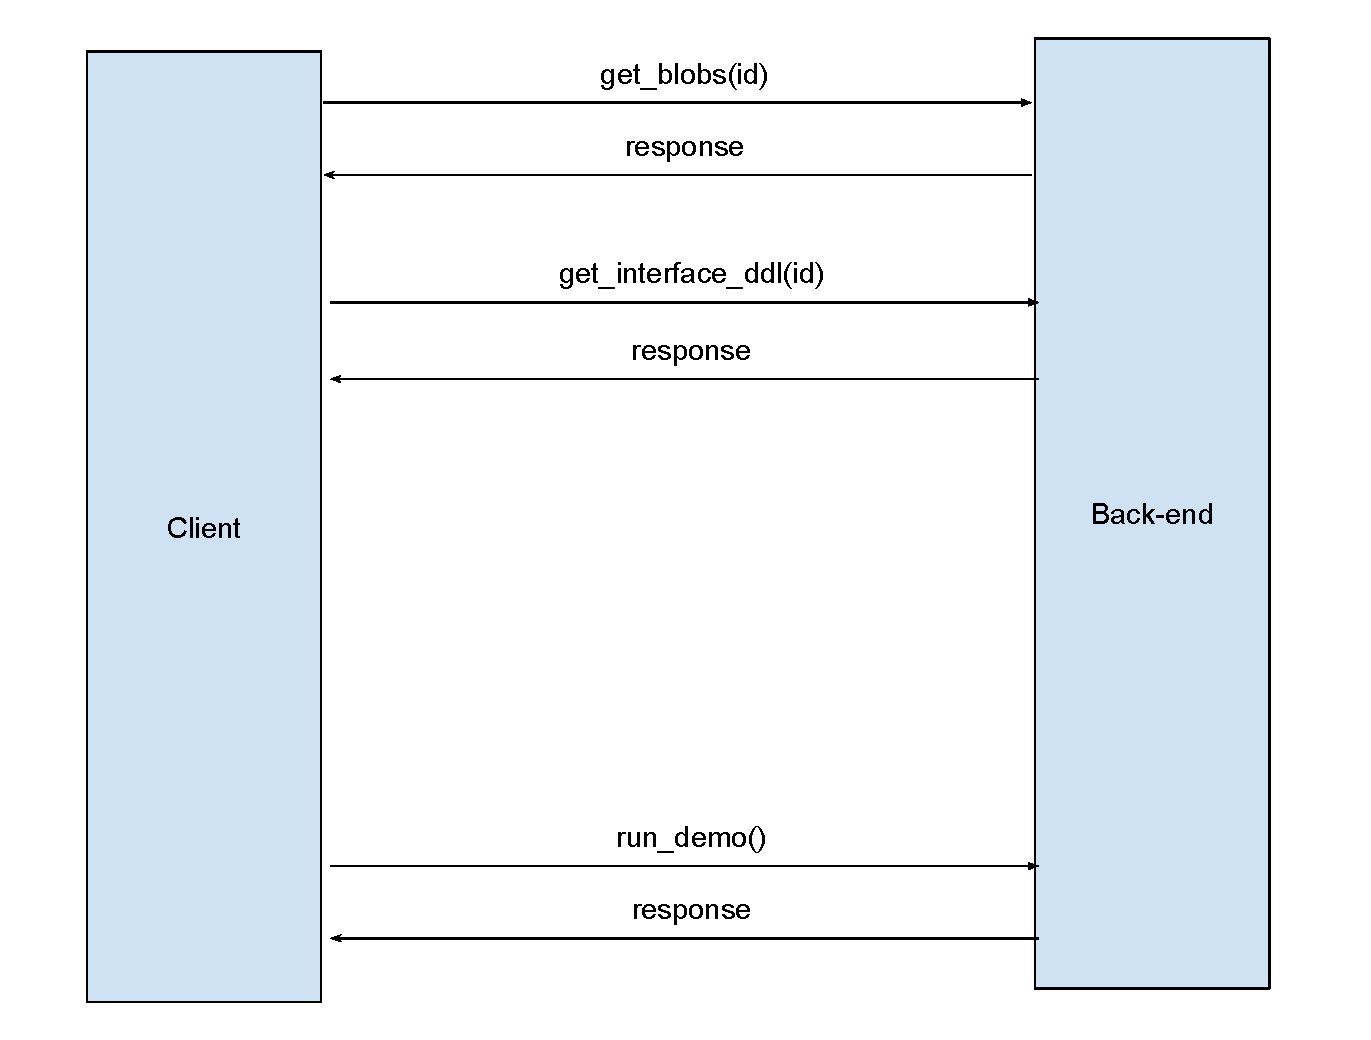
\includegraphics[width=\textwidth]{images/client_server_interaction}
	\caption{Client-server interation} 
	\label{fig:server_interaction}
\end{figure}

%--------------------------------------------------------------------------------

\section{Flow diagram}
When the application is loaded, the input module will locate the demo according to its ID. This ID is a get parameter from the URL.
Once the demo has this ID parameter, the main file, demo.js will load the different HTML files into the DOM. They have been divided 
into several files to improve maintainability and coupling.

After this process is done, the app will continue rendering the main section to the DOM, containing, in this case, the blobs viewer and 
the blob upload dialog. The information regarding the DDL and the blobs specification will be saved in sessionStorage once it has been retrieved by the asynchronous calls for easy access.

\begin{figure}[h]
	\centering
	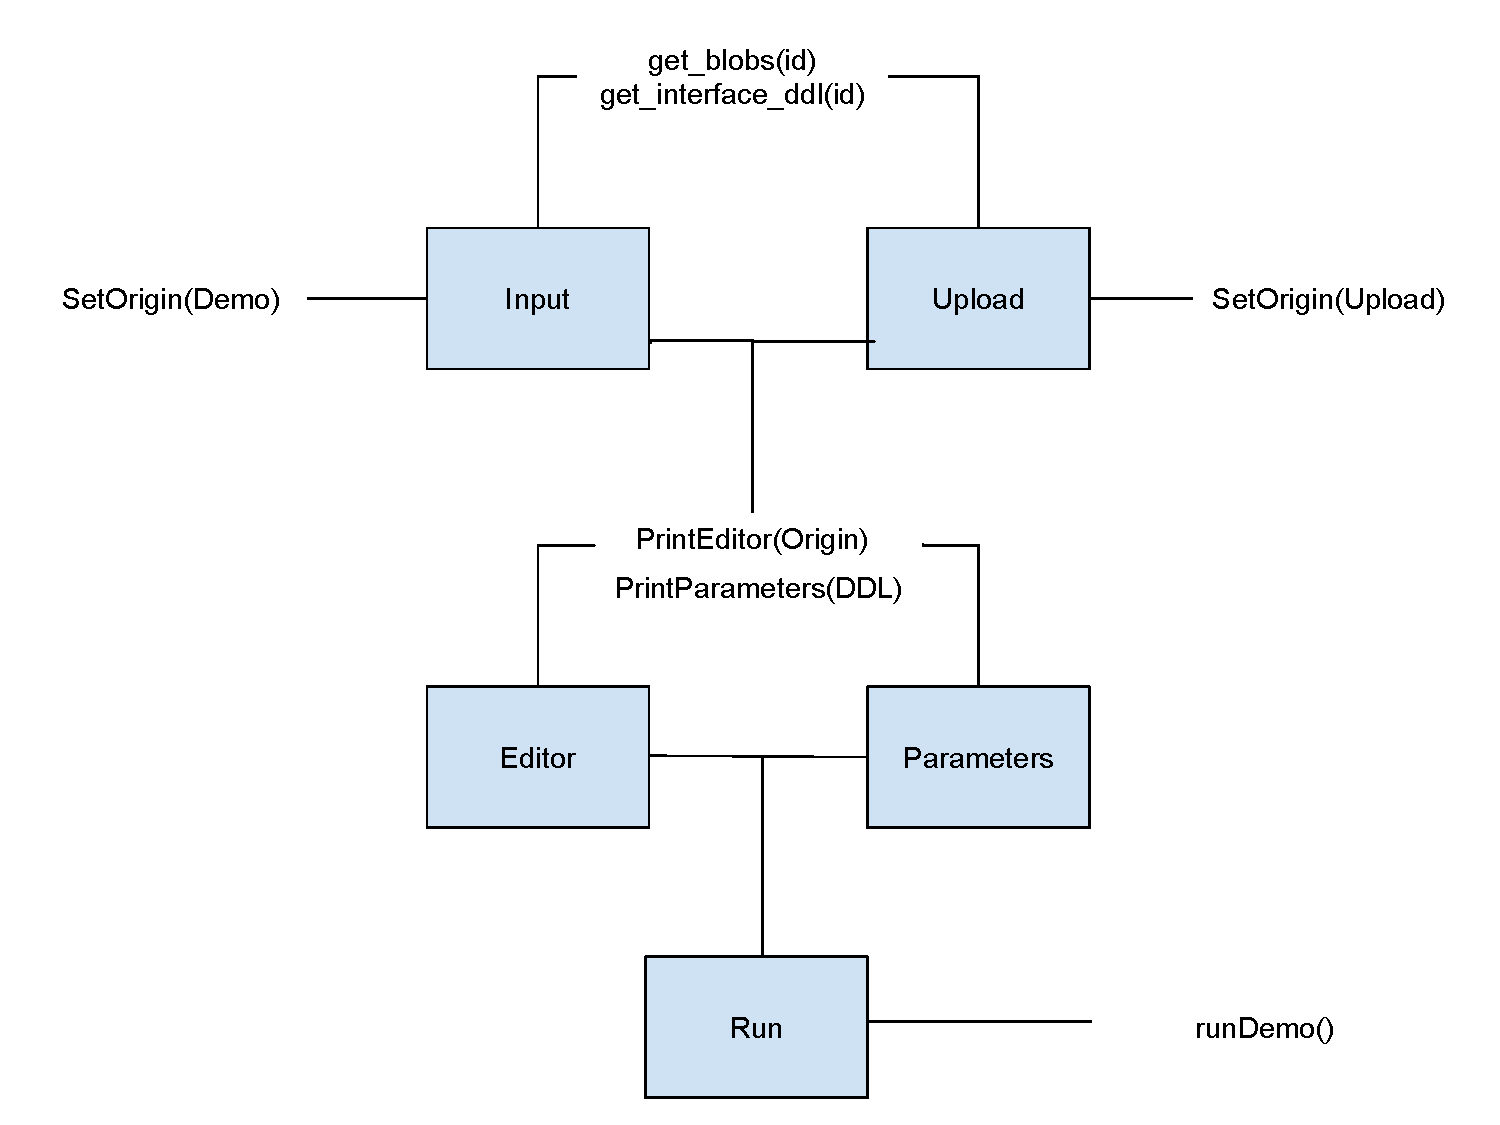
\includegraphics[width=\textwidth]{images/flow}
	\caption{Flow diagram} 
	\label{fig:flow_diagram}
\end{figure} 


As shown in figure  \ref{fig:flow_diagram}, either input or upload modules will pass 
information to the following modules. Each will set a variable in sessionStorage that will indicate if the user has chosen to 
upload blobs for the demo or a default blob from the list. If this variable is not set, it means the demo has no inputs defined 
in the DDL.

After the user chooses a blob, the editor and parameter modules will load independently and wait for changes. The Editor control 
will allow to either zoom, crop, and compare blobs if it is possible, as well as do masking operations when the demo requires it. 
The parameters will be modifiable according to the DDL specification values and will be stored in a variable in order to achieve 
parameter visibility dependence and to send this data when the run button is pressed.

After the user hits the run button an HTTP post will be executed to run the demo and send the necessary information and wait for 
a response. When the response is obtained it will either print the results interface or the error message.

%--------------------------------------------------------------------------------

\subsection{Sharing results}
Every time a demo is run, the URL will change to include the run key. This key allows the user to share the relatively short URL 
with anyone. Sharing will allow other users to see the parameters, results and inputs including crop information exactly just as the 
demo was executed by the original user. 

\subsection{Private mode}
This functionality allows the user to do a private execution of the demo. This makes the system not to record anything in the archives when running 
a demo. So nobody will see the execution results unless you share the URL with the execution key to someone. To activate private 
mode there is a checkbox in the lower part of the upload dialog.

\subsection{External modules}

The IPOL demo Web interface uses external libraries for extra functionalities.
Currently, it uses:

\begin{itemize}
\item Cropper.js: Cropper.js it is a simple image cropping JQuery plugin. It is used in the editor panel with the image blobs.
\end{itemize}

%--------------------------------------------------------------------------------

\subsection{Async calls}
The IPOL demo Web interface uses asynchronous calls to get the necessary information from the IPOL server.

The current version uses asynchronous calls for:
\begin{itemize}
\item Get the demo DDL: Used to show the inputs description and the upload modal in the Inputs panel, also uses this information to show the parameters.
\item Get blobs: Used to show the blobs in the inputs panel.
\item Run demo: It will send all the parameters needed to run the demo enclosed in the runData variable and will respond with either the results of 
the demo or an error response.
\end{itemize}

%--------------------------------------------------------------------------------

\subsection{Data types}
The IPOL platform supports images, audio and video files to use in demos. The new web interface 
allows choosing a set with any combination of images, audio and video. Depending on the data types and sets length options will vary. 
If a set contains multiple images, the user will be able to compare and make zoom using any image on the set. If the user chooses a set with only 
one image blob, options will depend on DDL limitations and will include zoom and crop features, as well as mask editing.

\section{Implementation of Features}
This section describes how particular features on the web interface are implemented.

%
\subsection{Execution recovery}
It is common that a researcher gets an interesting result after executing a demo with some particular input and parameters and want to share with a colleague. The first intuition is to simply copy the URL shown in the browser and ask the other persons to paste it in their own browser, to get the same page. Note that this is different from browsing the archive or to recover an archived experiment.

The IPOL webpage is AJAX dynamic and therefore this need that the web interface and the back-end do some extra work. The idea is to save the \emph{state} of the page after the execution, including the origin of the blobs used (uploaded original content or examples from the demo), the crop, parameters, and the results displayed. In general, any data needed to recover the same page state.

After the execution of the demo, the Core module saves the run request and the corresponding response into a {\tt execution.json} text file after the web interface requests the {\tt save\_execution} service. This file is saved at the temporal execution folder.
%
When the web interface needs to recover the state of the page it invokes the {\tt load\_execution} service of the Core along with the demo ID and the execution key. The Core reads the text file and sends back to the web interface all the information needed to put the demo page in the appropriate state.

The interaction diagram is shown in Fig. \ref{fig:execution_flow}.

\begin{figure}[h]
	\centering
	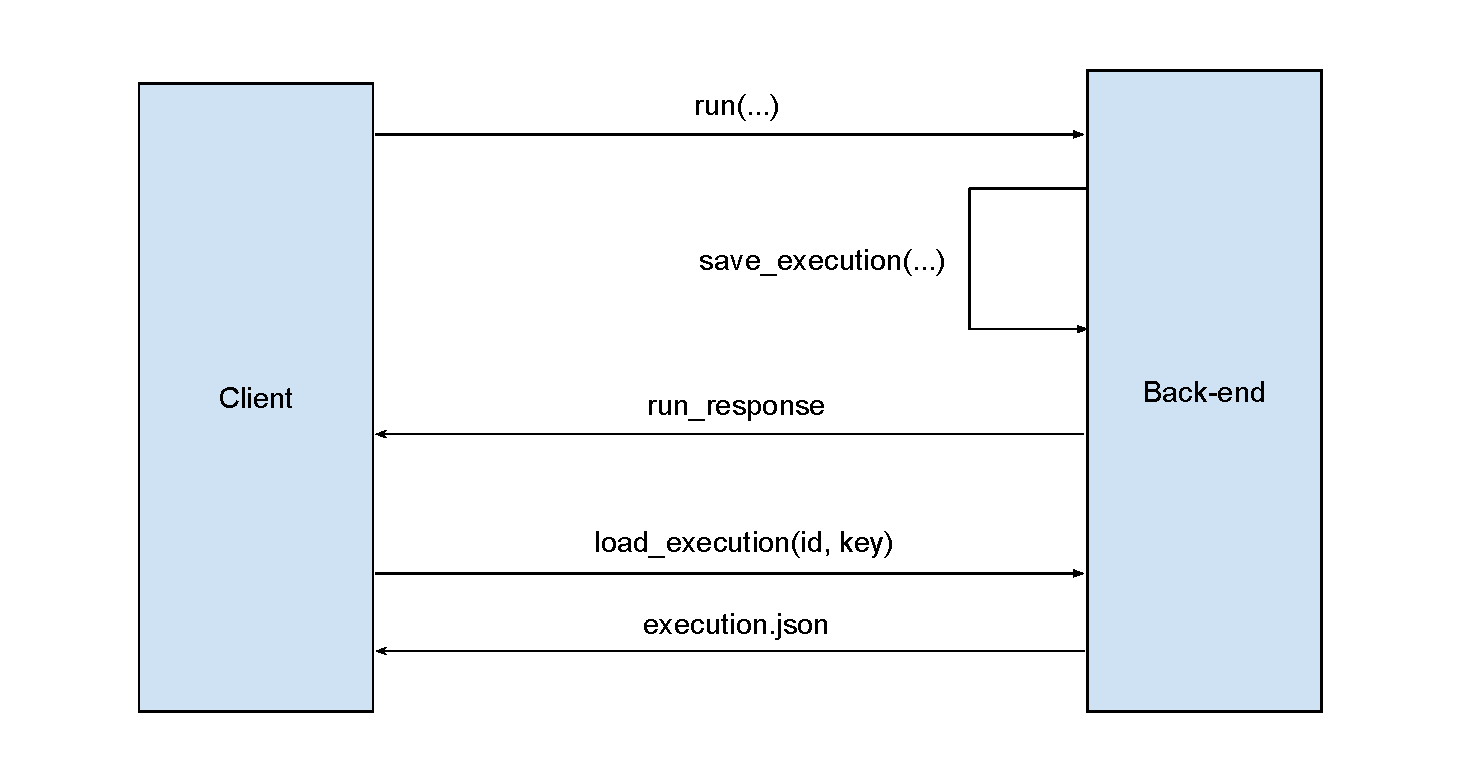
\includegraphics[width=\textwidth]{images/execution_flow}
	\caption{Execution flow diagram for the functionality of saving/recovering the state of the demo page.} 
	\label{fig:execution_flow}
\end{figure}

\subsection{Archive experiment reconstruction}
The purpose of this functionality is not only to show the experiment results but the demo page.

The user is able to reconstruct the experiment with the same inputs, parameters and results as the original experiment. The web interface sends a request to "/api/archive/get\_experiment?experiment\_id=XXX" to get all the needed information (for example, the images URLs or user parameters) to reconstruct the page in the same state after the execution. 

\bigbreak

There are two ways to reconstruct an experiment from the archive:
\begin{itemize}
	\item Clicking the button on the archive page of the specific experiment.
	\item Using the URL with the parameter  "archive=XXX". Useful to share results.
\end{itemize}

%\bibliographystyle{plain}
%\bibliography{biblio}

\end{document}
% End of document
